\documentclass[12pt]{article}
\usepackage[english]{babel}
\usepackage[utf8]{inputenc}
\usepackage{amssymb}
\usepackage{amsmath}
\usepackage{amsthm}
\usepackage{hyperref}
\usepackage{tikz}
\usepackage{hyperref}
%\usetikzlibrary{automata,positioning}
\usepackage{graphicx}
\graphicspath{ {images/} }
\usepackage[linewidth=1pt]{mdframed}
%\usepackage{algorithm}
%\usepackage{algpseudocode}
\usepackage{fancyhdr}
\usetikzlibrary{decorations, decorations.text,}

\topmargin=-0.45in
\evensidemargin=0in
\oddsidemargin=0in
\textwidth=6.5in
\textheight=9.0in
\headsep=0.25in

%\pagestyle{fancy}
%\lhead{Name: Anjana Tiha}
%\chead{}
%\rhead{Information Retrieval and Web Search(COMP 8130)}
%\lfoot{}
%\cfoot{Page \thepage}
%\rfoot{\today, Fall, 2017}

\begin{document}

	\begin{titlepage}
		
		\begin{center}
			\begin{large}
			\vspace*{11em}
			\textbf{
			Homework\textendash 7\\
			\vspace{2em}
			Course Name: Information Retrieval/Web Search(COMP 8130)\\
			\vspace{0.5em}
			Course Instructor: Professor Vasile Rus\\
			\vspace{2em}
			Submitted By\\
			\vspace{1em}
			Student Name: Anjana Tiha\\
			UID: U00619942\\
			Date: 11/22/2017\\
			}
			\end{large}

		\end{center}
		
	\end{titlepage}
	\newpage
\section*{Problem 1 [30 points].}
Develop a retrieval program that takes as input an user query in the form of a set of keywords, uses the inverted index to retrieve documents containing
at least one of the keywords, and then ranks these documents based on
cosine values between query vector and document vectors. The output should be a ranked list of documents with links to the original documents, i.e. URLs to the original documents on the web.
\section*{Answer 1:}
\subsection*{Functionality : }
Program takes query search string as input and returns most relevant url from analyzing previously collected 10,000 unique web documents from "memphis.edu" domain where each collected document contains more than 50 tokens after preprocessing.
\subsection*{Method : }
\subsubsection*{Query Processing}
Added Query processing functionality along with TF-IDF vector generation of collected 10000 documents.
For query Processing:
Preprocessed query simmilar to document corpus processing:
\begin{enumerate}
\item Takes input string for query. 
\item Preprocesses the query string by removing the following: 
	\begin{itemize}
		\item[-] digits
		\item[-] punctuation
		\item[-] stop words (used the generic list available at ...ir-	websearch/papers/english.stopwords.txt)
		\item[-] uppercase
		\item[-] morphological variations
	\end{itemize}
\item Tokenized query string.
\item Generetaed TF-IDF vector from query.
\item Calculate cosine similarity between TF-DF vector of document corpus and query string. 
\item Ranks the cosine similarity of document and query in descending order. 
\item Show the corresponding urls for matching ranked documents from most similar to least.
\end{enumerate}
\subsubsection*{TF-IDF of Document Corpus}
Generated TF-IDF of document corpus from text collected from 10,000 web documents. Generated hashmap in format map\{word\}\= \{{file name\}= current word count\} in current file. Also maintained fields for maximum word count for a word in a file along with total word count. Another hashmap had (file, word: single word count in this file). This hashmaps were saved for later query similarity calculation. 
\section*{Problem 2 [20 points].}
Develop a web interface to the program above.
\subsection*{Web Interface}
Developed web interface using Django open-source web framework.\\
To see search using the web interface, please install Django web framework.\\\\
Steps: 
\begin{enumerate}
\item Install pip for python if not installed already.
\item Move to python directory or scripts directory in Anaconda.
\item Please enter  -"pip install Django" for installing Django.
\end{enumerate}
To open project in web interface:
\begin{enumerate}
\item To runserver for current project go to project folder "search\_engine\_website" where manage.py file is located.
\item Open command prompt in the directory of manage.py and type manage.py  preceded by python.exe location and python in the follwoing manner:
\item \path{C:\Users\Anjana\Anaconda3\python manage.py runserver
server}
\item \path{(format - >location for python.exe+python+ manage.py)}
\item To view web interface for search engine go to http://127.0.0.1:8000/
\end{enumerate}
\section*{Files:}
\begin{itemize}
\item search engine website contains all the documents after preprocessing, and hashmaps from doc to url map and other tfidf vector for document and query.
\item search\_engine.py is the main search engine file.
\end{itemize}
\section*{Document link:}
Google Drive Links:\\
\url{https://drive.google.com/open?id=1JOHK4UHuzLB4a6CaN8eAookPj48v-fJJ}
\section*{Figures}
\begin{figure}[!ht]
\caption{Search Engine Interface}
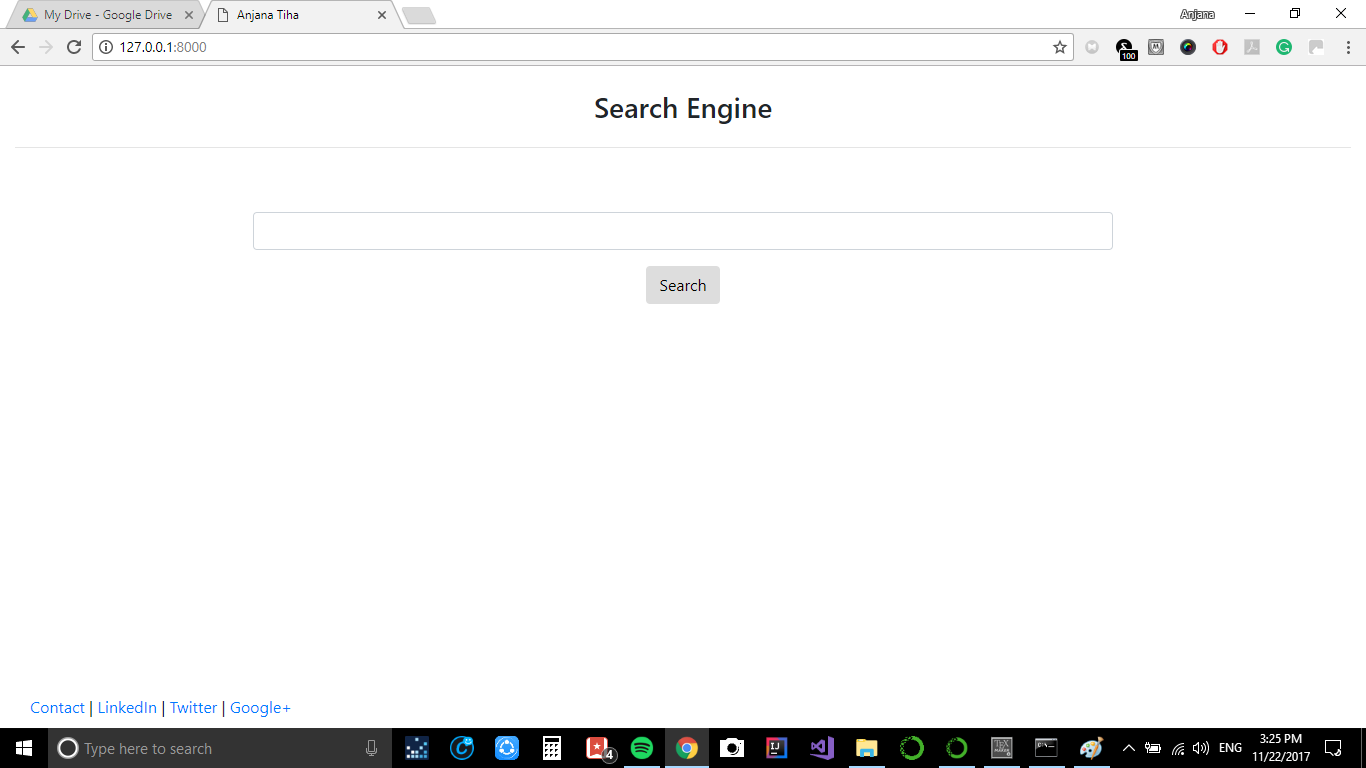
\includegraphics[scale=.5]{main}
\end{figure}
\begin{figure}
\caption{Search Engine Interface With Results}
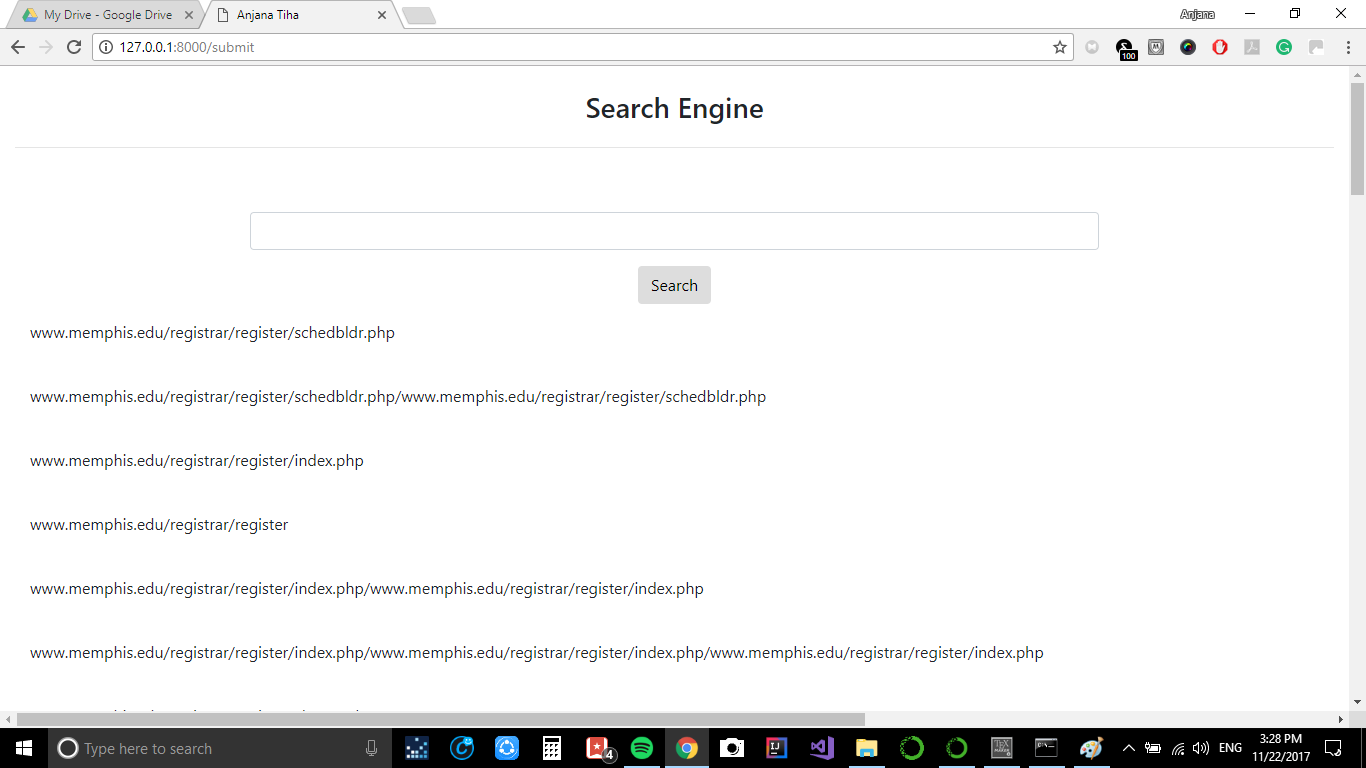
\includegraphics[scale=.5]{search}
\end{figure}
\end{document}

